% begin module volumes-ex2
\begin{frame}
\begin{example}[Example 2, p. 440]
Find the volume of the solid obtained by rotating about the $x$-axis the region under the curve $y = \sqrt{x}$ from $0$ to $1$.
\begin{itemize}
\item<8->  The cross-sections of this solid are all circles.
\item<9->  The circular cross-section through the point $(x, 0)$ has radius $\sqrt{x}$.
\item<10->  The area of the cross-section is \alert<handout:0| 10-11>{$A(x) = $ \uncover<11->{$\pi (\sqrt{x})^2$}} \uncover<12->{$ = \pi x$.}
\item<13->  The volume of a single approximating section is $A(x) \Delta x = \pi x \ \Delta x$.
\item<14->  The solid lies between $0$ and $1$, so its volume is
\end{itemize}
\begin{columns}[c]
\column{.4\textwidth}
\begin{center}
\only<handout:0| 1>{%
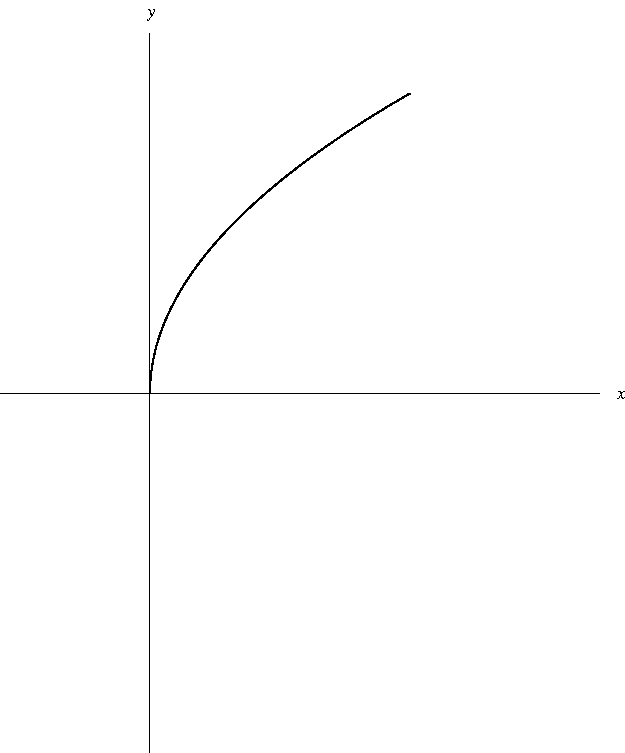
\includegraphics[height=3.5cm]{volumes/pictures/06-02-ex2a.pdf} %
}%
\only<handout:0| 2>{%
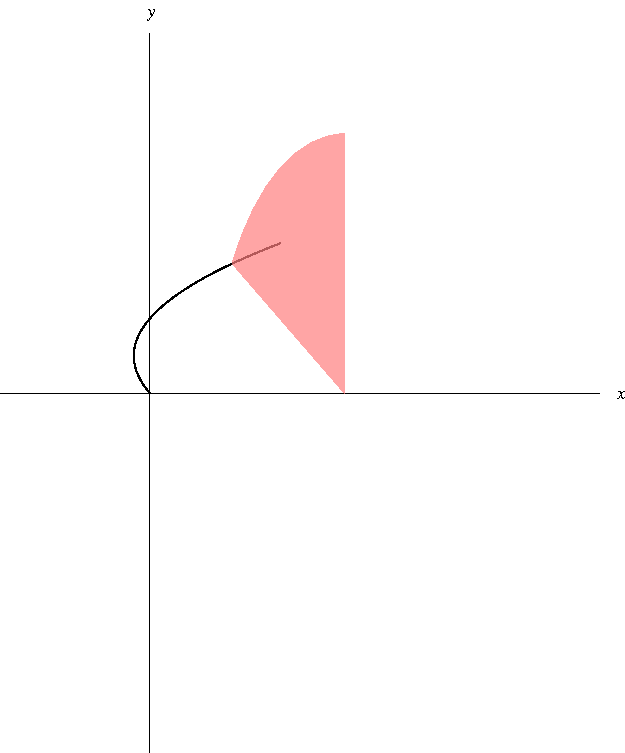
\includegraphics[height=3.5cm]{volumes/pictures/06-02-ex2b.pdf} %
}%
\only<handout:0| 3>{%
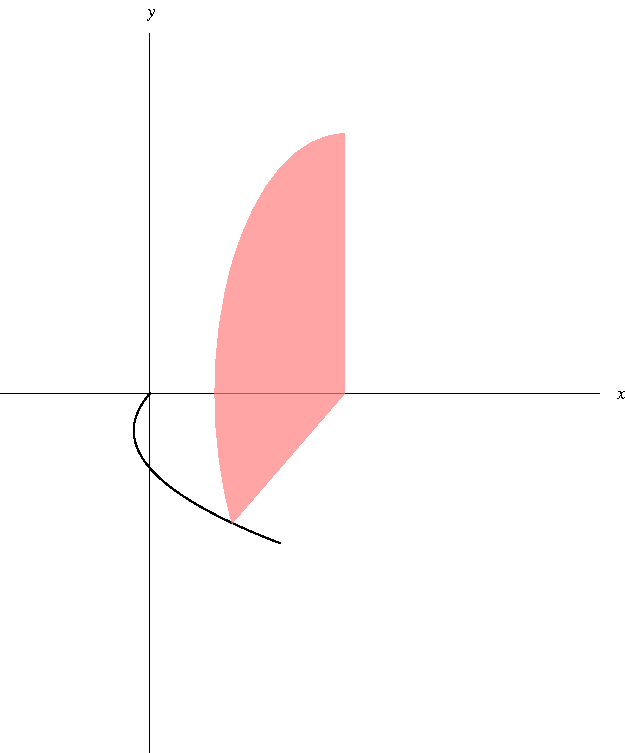
\includegraphics[height=3.5cm]{volumes/pictures/06-02-ex2c.pdf} %
}%
\only<handout:0| 4>{%
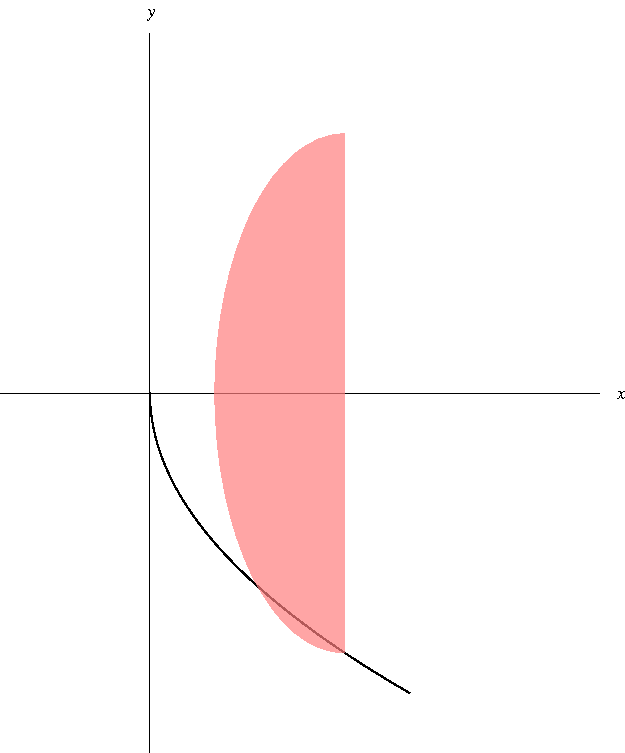
\includegraphics[height=3.5cm]{volumes/pictures/06-02-ex2d.pdf} %
}%
\only<handout:0| 5>{%
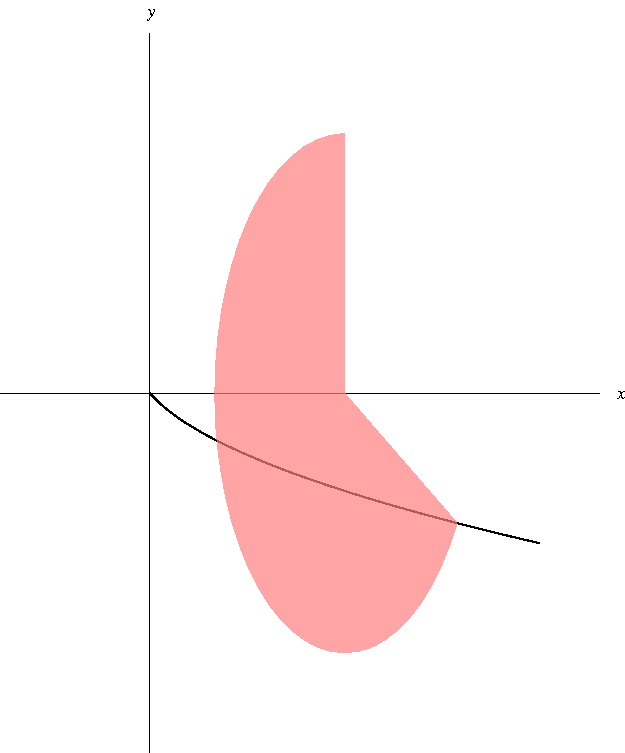
\includegraphics[height=3.5cm]{volumes/pictures/06-02-ex2e.pdf} %
}%
\only<handout:0| 6>{%
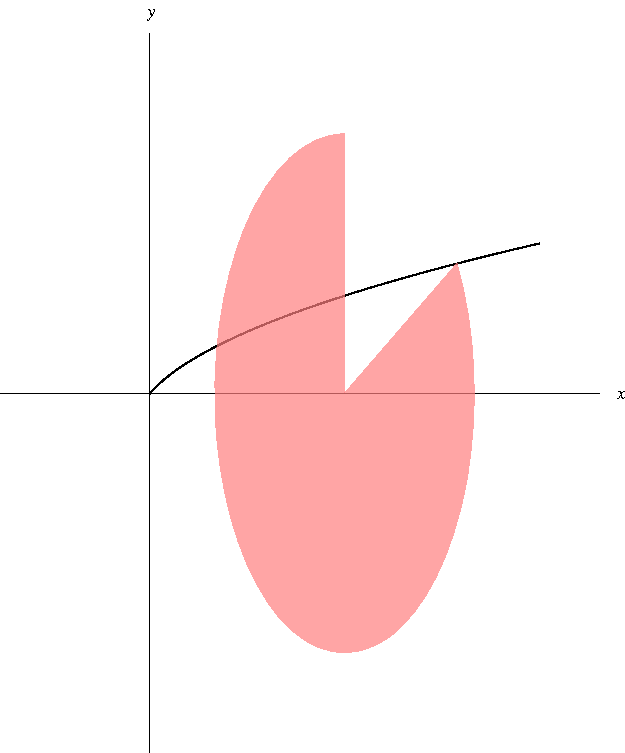
\includegraphics[height=3.5cm]{volumes/pictures/06-02-ex2f.pdf} %
}%
\only<7->{%
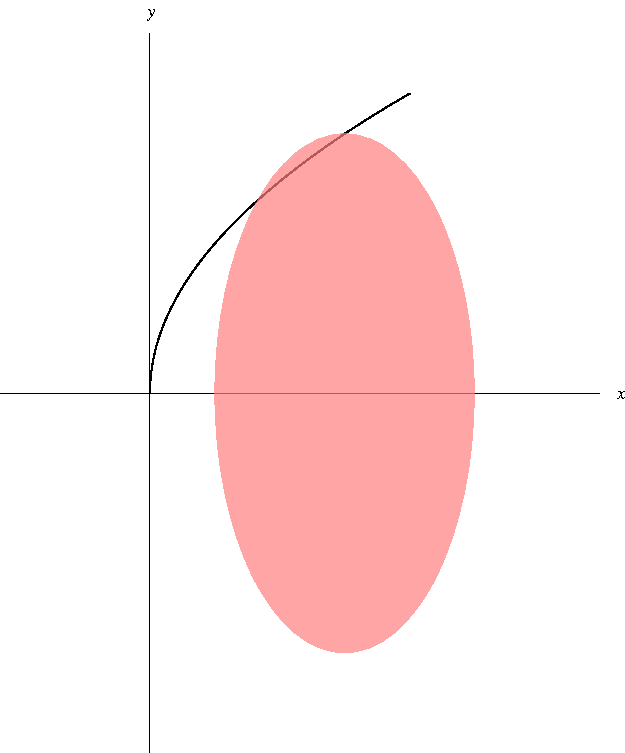
\includegraphics[height=3.5cm]{volumes/pictures/06-02-ex2g.pdf} %
}%
\end{center}
\column{.6\textwidth}
\abovedisplayskip=0pt
\belowdisplayskip=0pt
\abovedisplayshortskip=0pt
\belowdisplayshortskip=0pt
\begin{align*}
\uncover<14->{%
V%
}%
& \uncover<14->{ = } %
\uncover<14->{%
\int_0^1 A(x) \ \diff x%
}%
 \uncover<15->{ = } %
\uncover<15->{%
\int_0^1 \pi x \ \diff x%
}\\%
& \uncover<16->{ = } %
\uncover<16->{%
\left[ \pi \frac{x^2}{2}\right]_0^1%
}%
 \uncover<17->{ = } %
\uncover<17->{%
\frac{\pi}{2}%
}%
\end{align*}
\end{columns}
\end{example}
\end{frame}
% end module volumes-ex2
